\chapter{Implementación}

En este capítulo se detalla la implementación de la plataforma desarrollada, describiendo las decisiones técnicas, herramientas y metodologías empleadas para materializar los objetivos planteados. La arquitectura del sistema se fundamenta en la separación clara entre el backend, responsable del procesamiento de datos y la lógica principal de la aplicación, y el frontend, encargado de la presentación e interacción con el usuario. Esta aproximación modular facilita el mantenimiento, escalabilidad y futuras extensiones del sistema.

\begin{figure}[H]
  \centering
  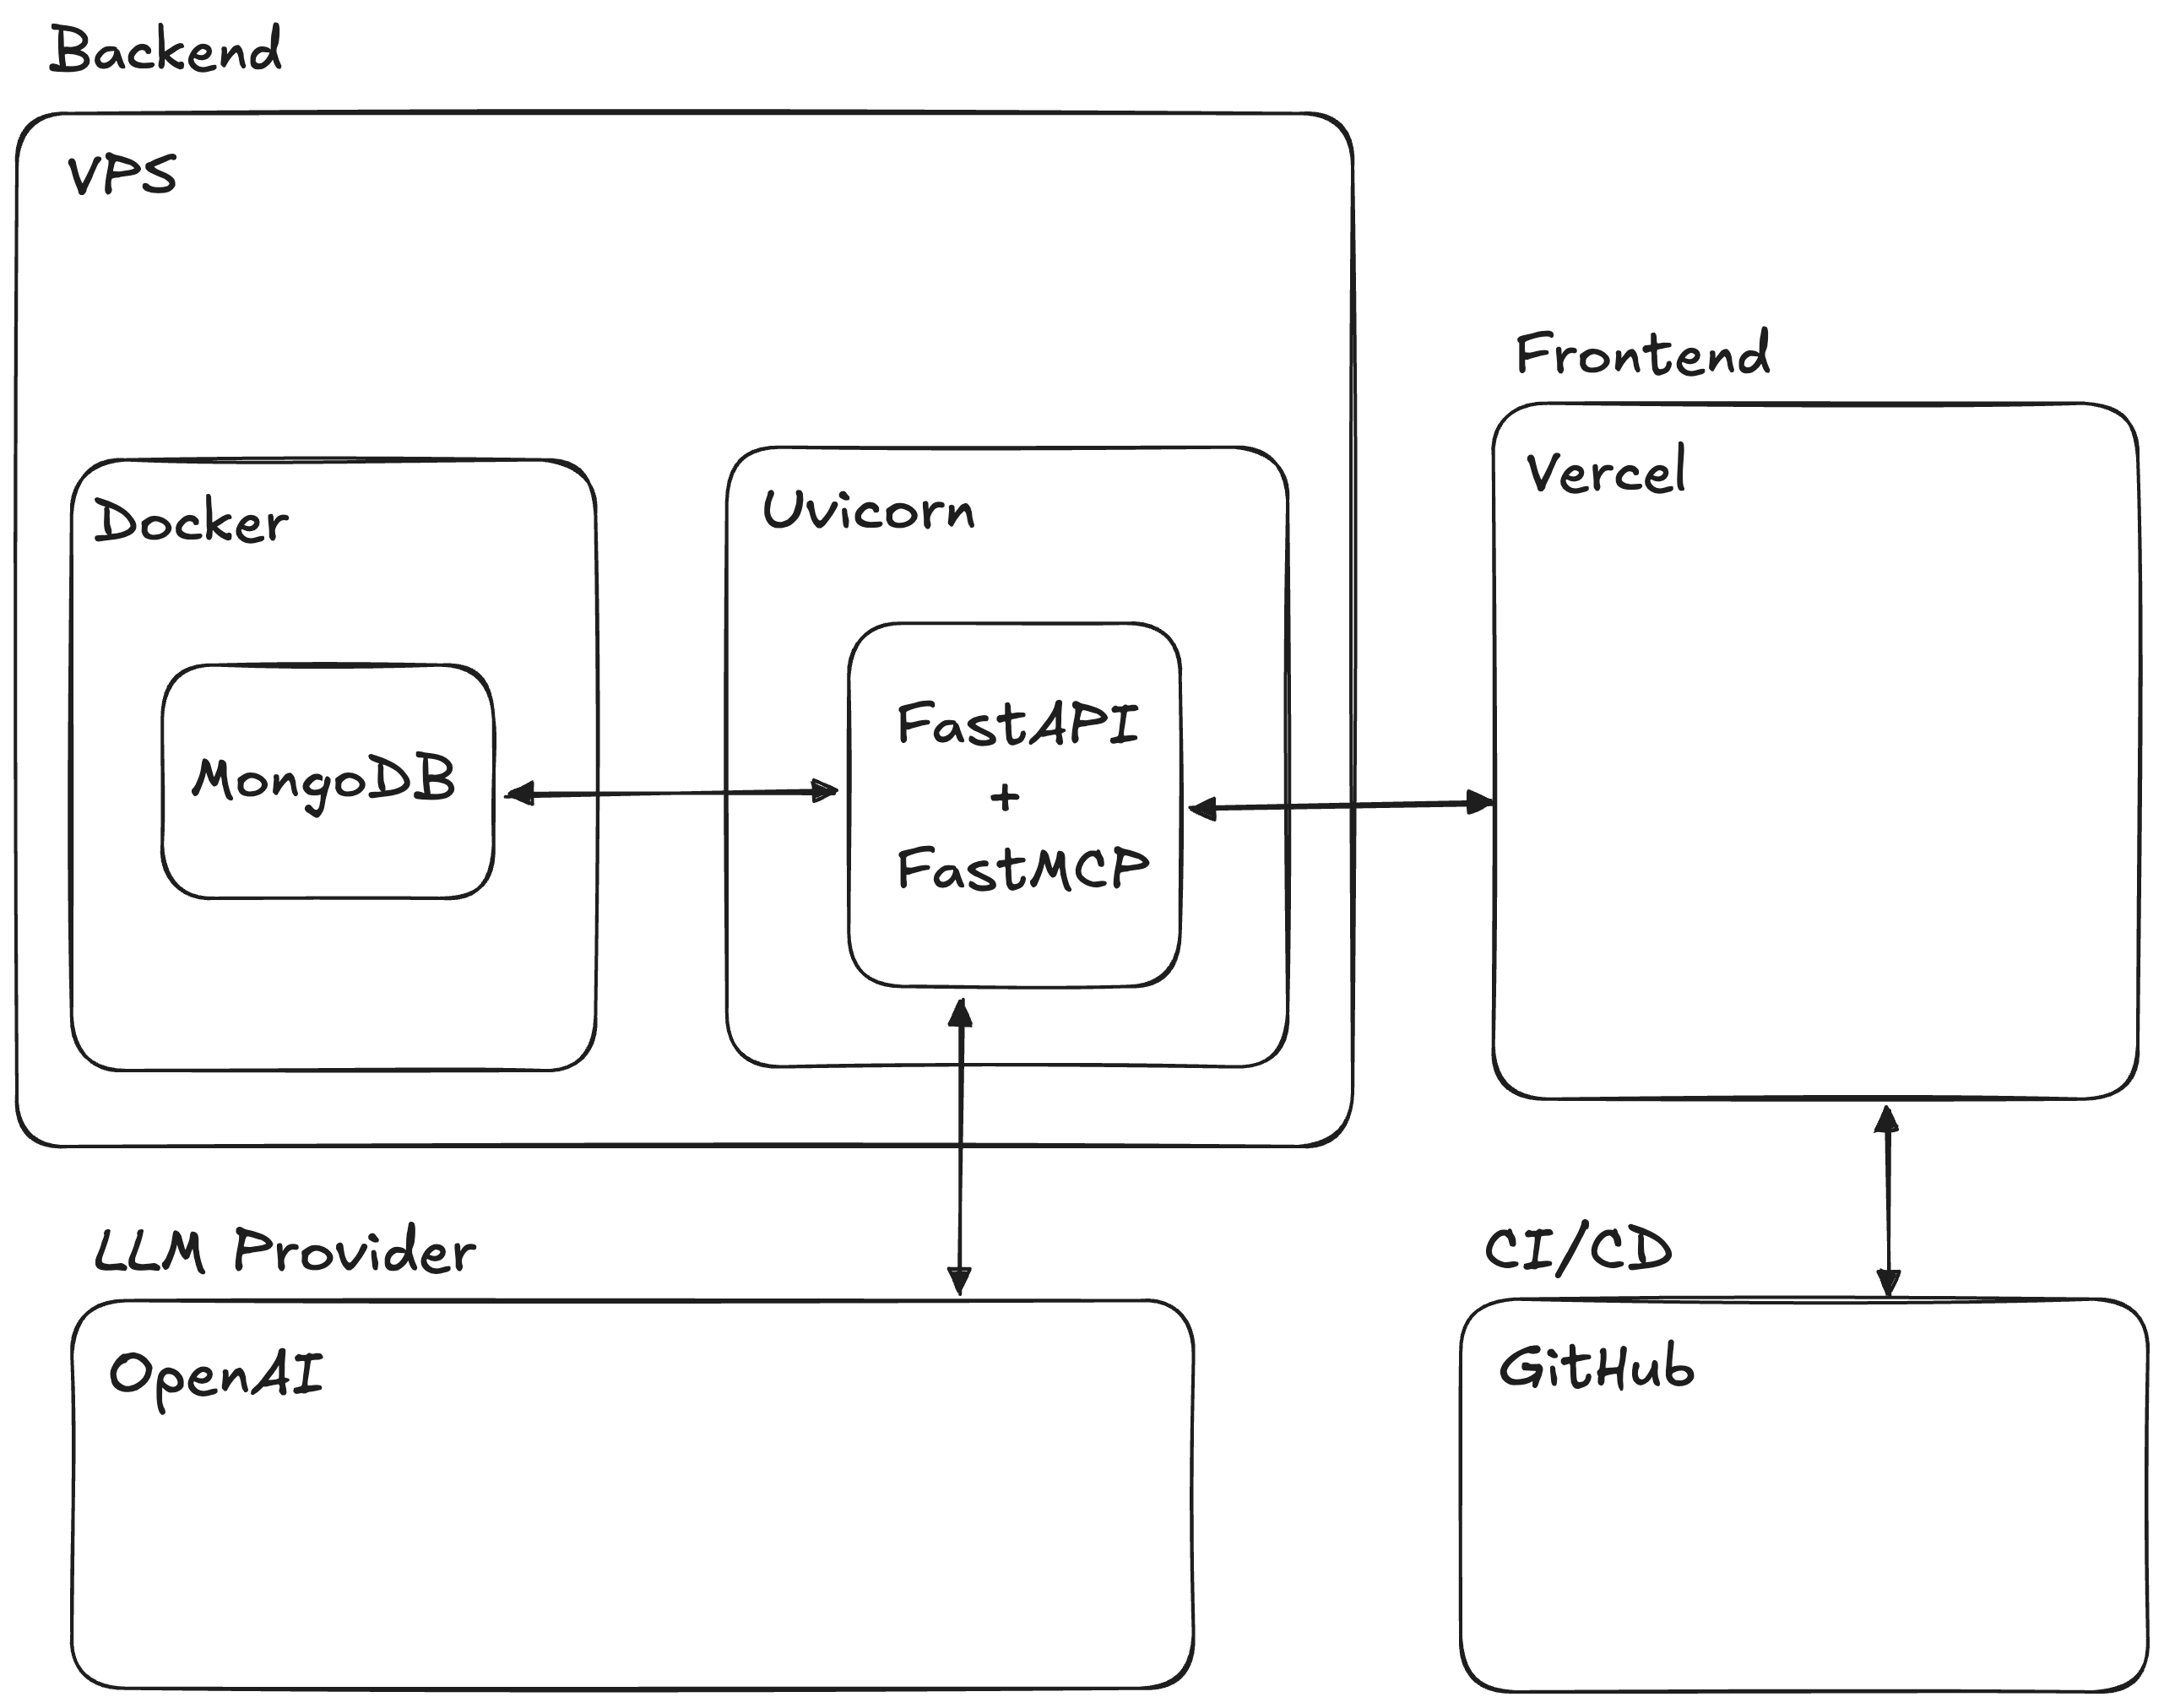
\includegraphics[width=0.9\textwidth]{imagenes/arch1.png}
  \caption{Arquitectura de la aplicación}
  \label{fig:arch1}
\end{figure}

\section{Backend}

El backend constituye el núcleo de la lógica de este trabajo. Se puede dividir en dos elementos: la base de datos MIMIC-IV almacenada en MongoDB con Docker, y la API RESTful con FastAPI que consulta datos, los procesa y los devuelve al cliente. Todo se aloja en un servidor personal y se accede por HTTPS gracias a Cloudflare Tunnels.

%\subsection{Almacenamiento de MIMIC-IV en MongoDB}
\subsection{MIMIC-IV en MongoDB}


Una de las tareas técnicas fundamentales del proyecto ha sido la migración del conjunto de datos desde su formato original en CSV a una base de datos MongoDB. MIMIC-IV se distribuye como un conjunto de archivos CSV comprimidos organizados en dos módulos principales: \texttt{hosp} (datos hospitalarios) e \texttt{icu} (datos de cuidados intensivos), junto con diccionarios de códigos y metadatos complementarios.


El proceso de migración se implementó mediante scripts de Python utilizando la librería \texttt{pandas} para la lectura de archivos CSV y \texttt{pymongo} para la inserción en MongoDB. Cada fila del CSV se convierte en un archivo JSON en MongoDB, cada columna es un campo del documento, y cada archivo CSV completo acaba siendo una colección de documentos. El procesamiento se hizo por chuncks para evitar el desbordamiento de memoria, que fue un problema recurrente debido a la cantidad masiva de datos.


Tras la importación, resultaron las siguientes colecciones:




Para el despliegue de MongoDB se utilizan dos contenedores Docker, en distintos puertos, uno para la versión demo del conjunto de datos, y otro para la versión completa, facilitando la realización de pruebas. Como apoyo al desarrollo, y también en forma de contenedores, se despliegan las herramientas de interfaz gráfica: Portainer para Docker\cite{portainer_ce} y Mongo Express para las bases de datos\cite{mongo_express}. 

\begin{figure}[H]
  \centering
  \fbox{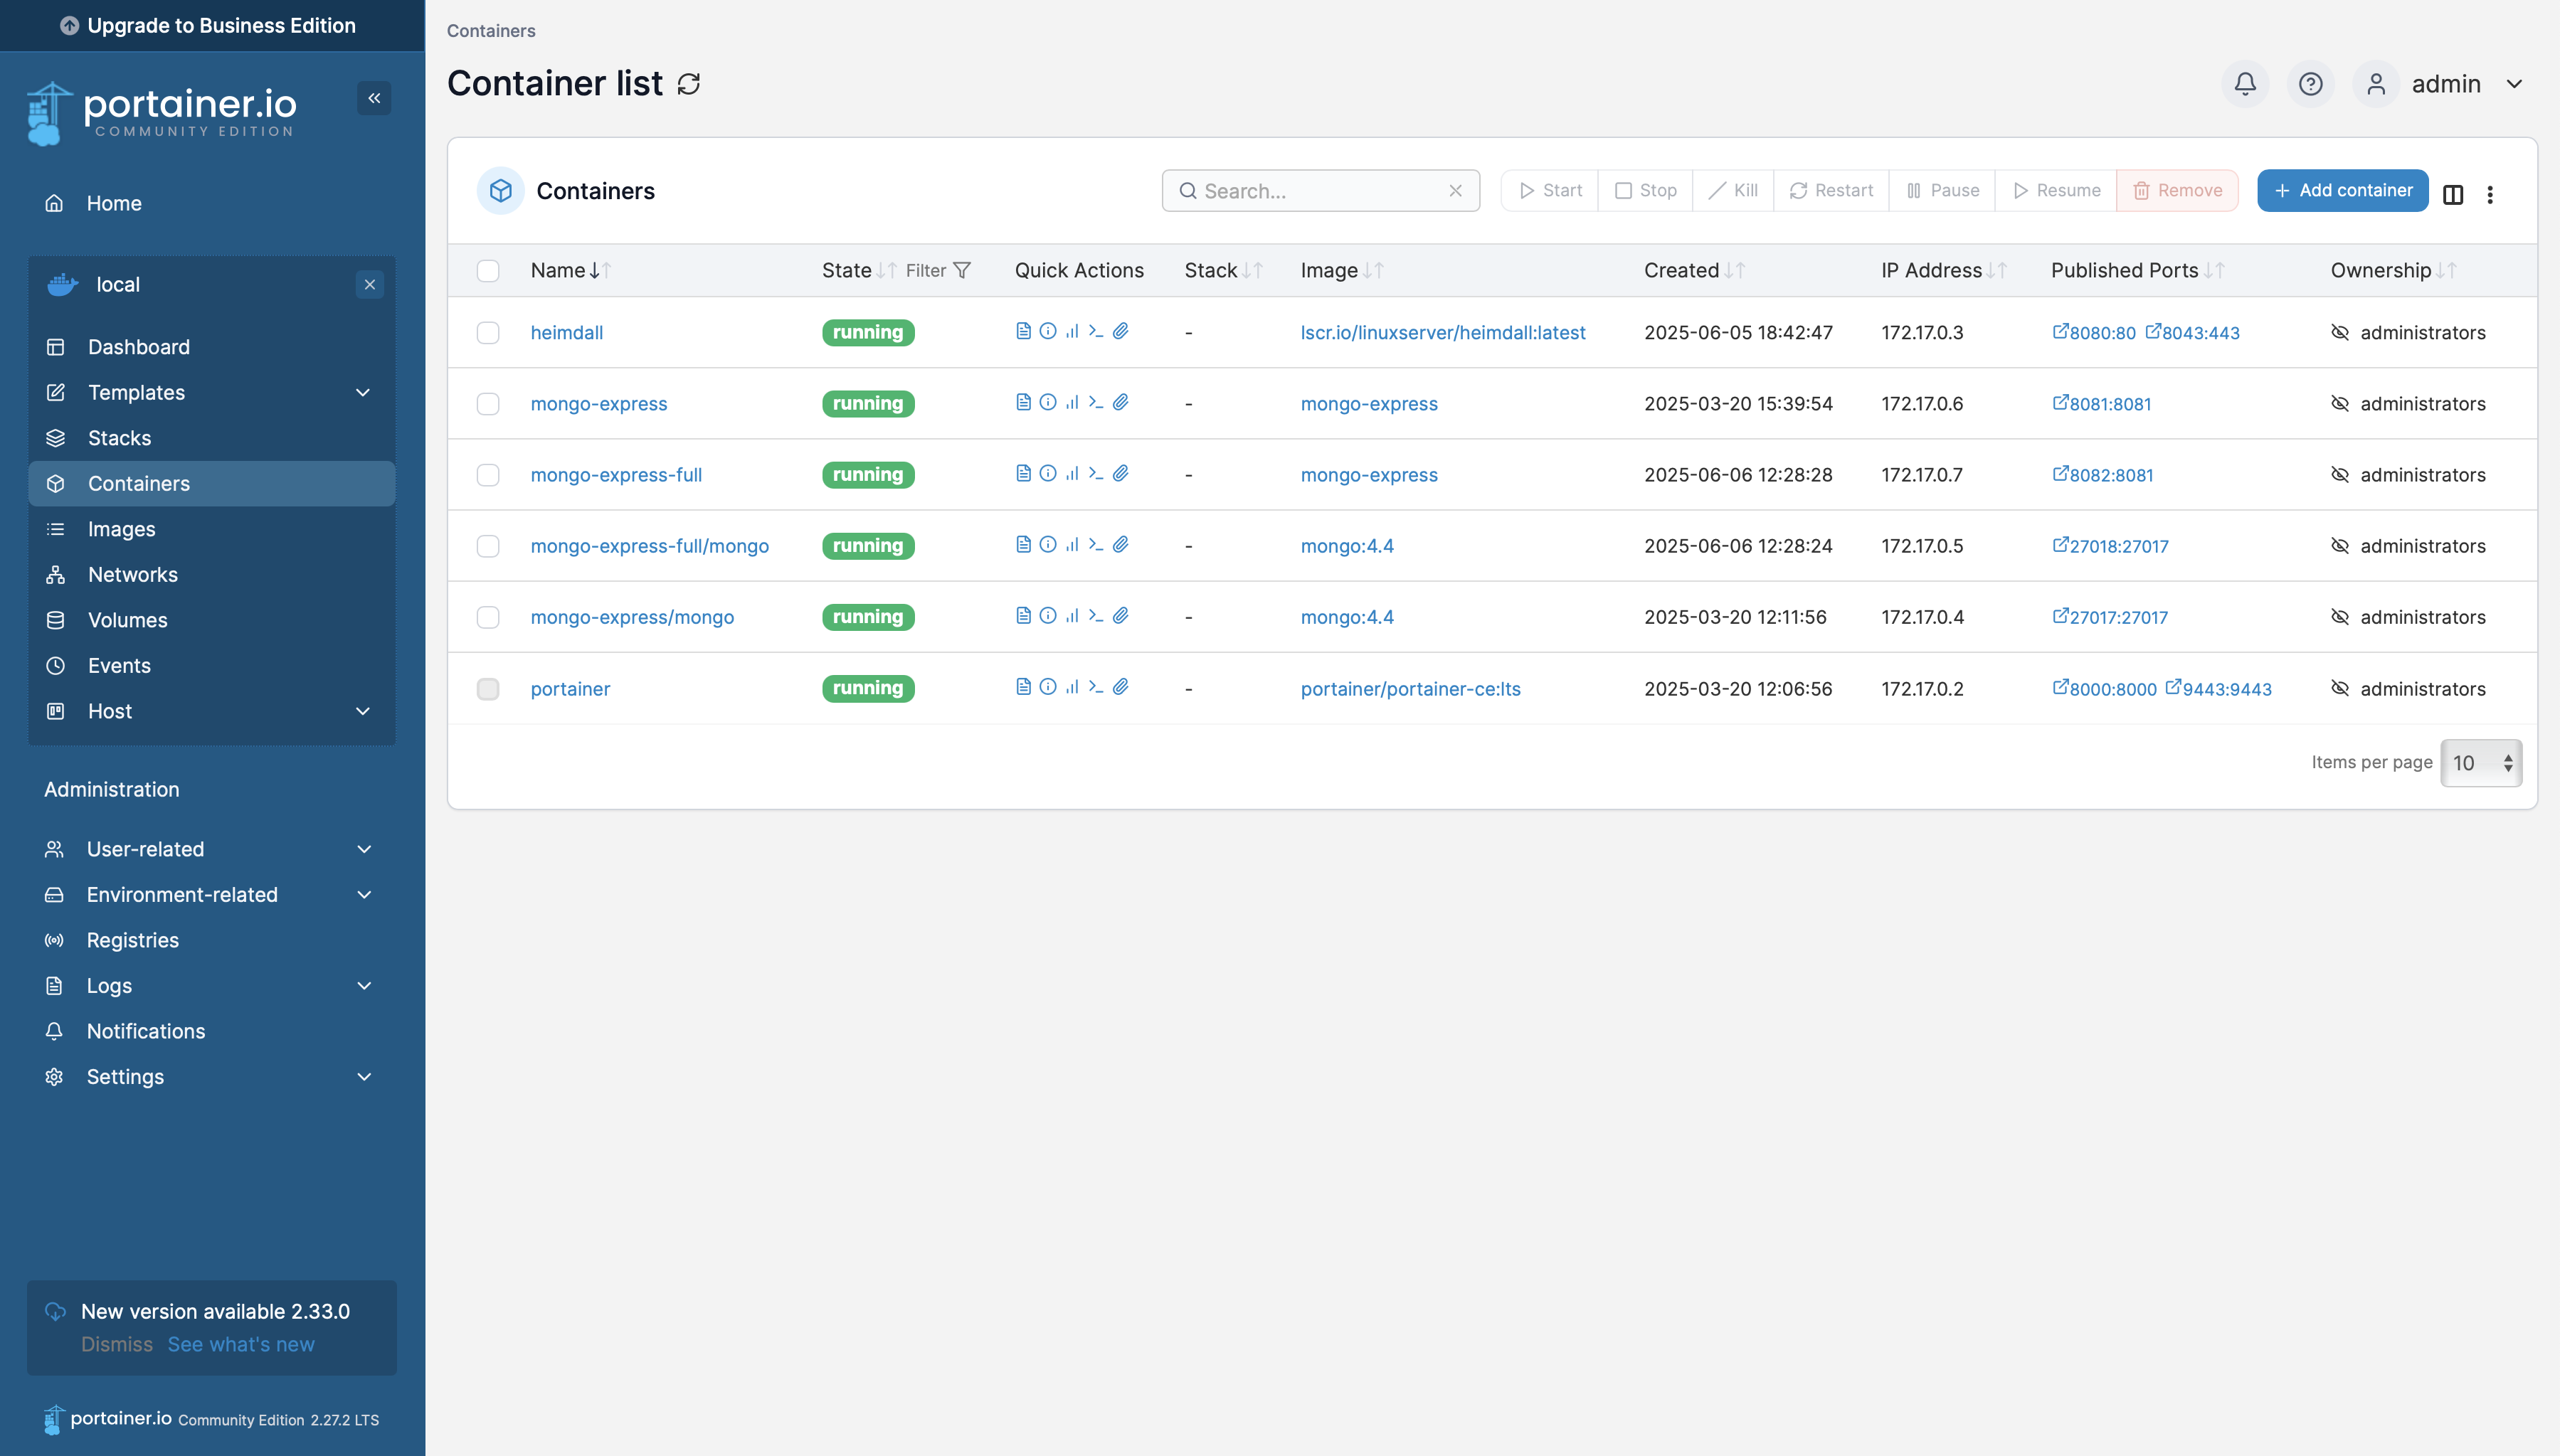
\includegraphics[width=1\textwidth]{imagenes/screenshot1.png}}
  \caption{Captura de pantalla de Portainer}
  \label{fig:screenshot1s}
\end{figure}


\begin{figure}[H]
  \centering
  \fbox{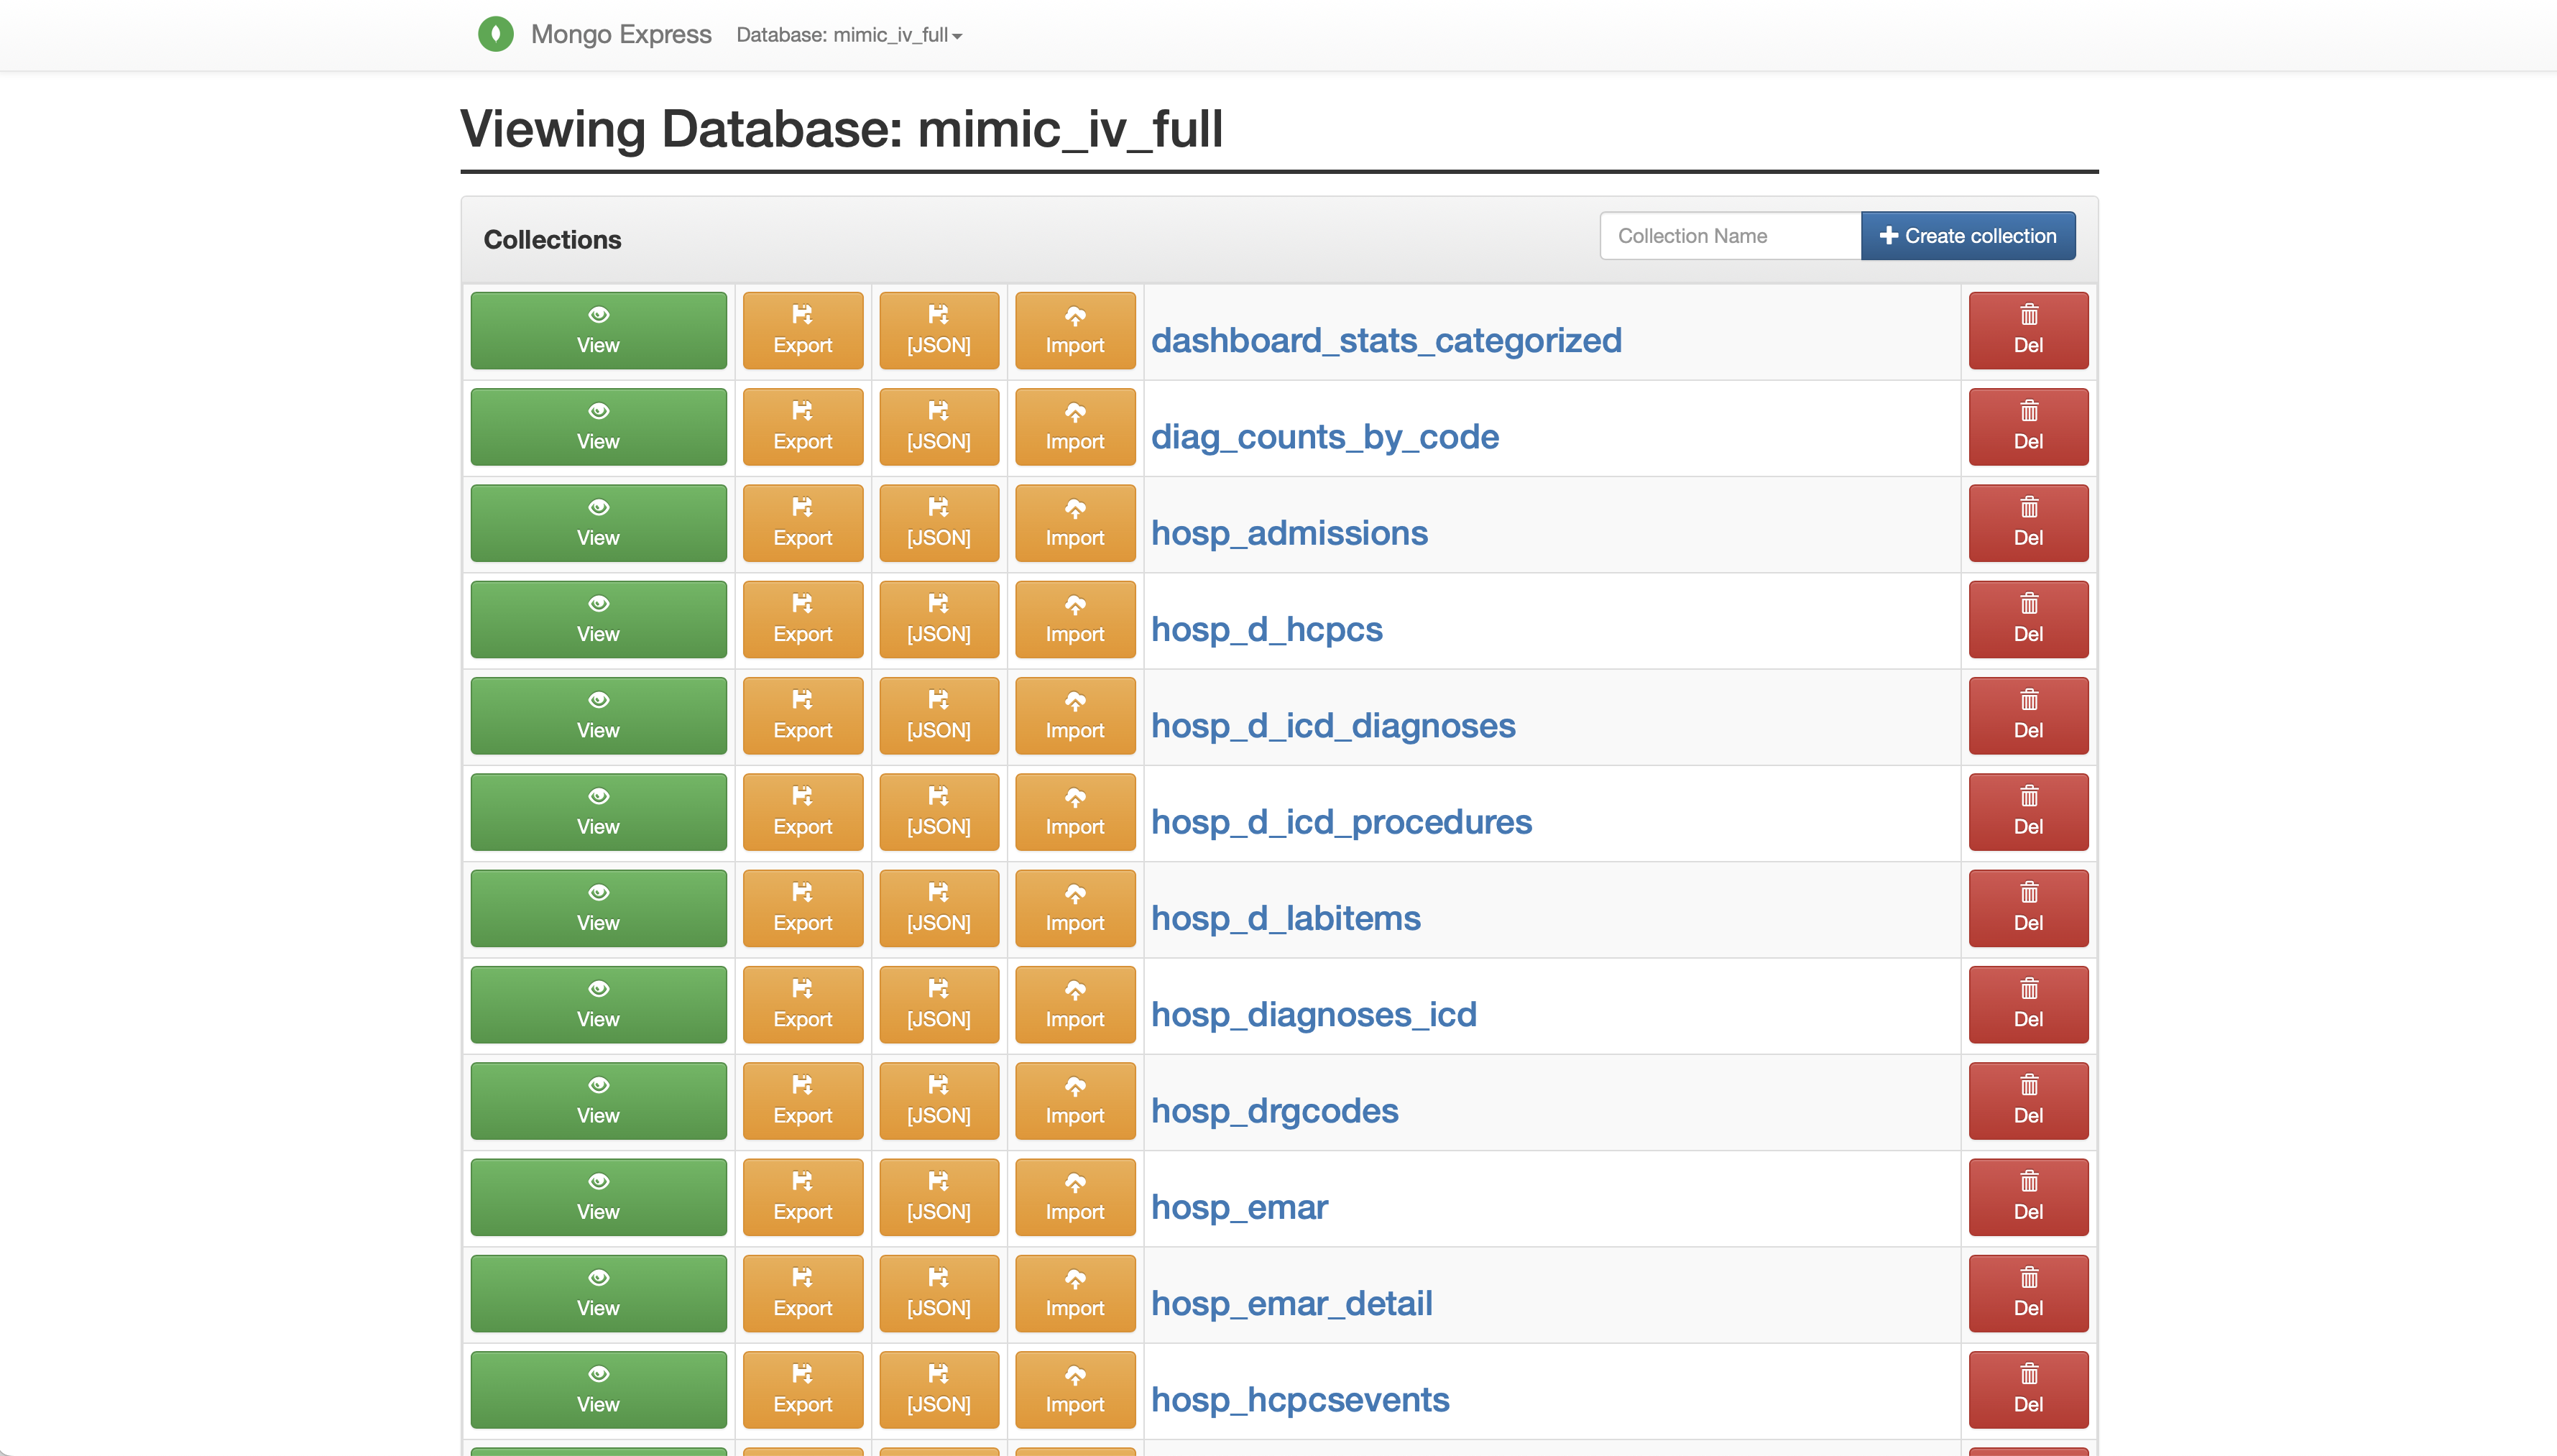
\includegraphics[width=1\textwidth]{imagenes/screenshot2.png}}
  \caption{Captura de pantalla de Mongo Express}
  \label{fig:screenshot2}
\end{figure}


\subsection{API RESTful}

La API que obtiene, procesa y sirve los datos está construida sobre FastAPI, un framework moderno que combina alto rendimiento con una sintaxis intuitiva y generación automática de documentación. Para separar responsabilidades, el código se estructura de la siguiente forma:

\begin{itemize}
\item \textbf{Capa de datos:} El módulo \texttt{db/mongo.py} encapsula la conexión a MongoDB y proporciona funciones de utilidad.
\item \textbf{Capa de rutas:} Organizadas por funcionalidad en el directorio \texttt{routes/}, incluyen endpoints para pacientes, dashboard, gráficos y chat.
\item \textbf{Capa de aplicación:} El archivo principal \texttt{main.py} configura la aplicación, middleware CORS y el enrutamiento.
\end{itemize}

Utilizamos Uvicorn como servidor ASGI (Asynchronous Server Gateway Interface) que escuchará las peticiones a los endpoints. 

(...completar con las demas cosas que se usen para la IA)

(...poner imagen esquemita de los archivos orden y tal?)


\subsection{Inteligencia Artificial}

La integración de inteligencia artificial en esta plataforma se fundamenta en la utilización de grandes modelos de lenguaje (LLMs) para facilitar la consulta y análisis de datos clínicos en lenguaje natural. Esta aproximación permite que usuarios sin conocimientos técnicos avanzados puedan extraer información valiosa de la base de datos MIMIC-IV mediante conversaciones naturales, eliminando la barrera técnica que tradicionalmente requería conocimientos de SQL o programación.

Para este proyecto se ha elegido trabajar con los modelos de texto de OpenAI, específicamente GPT-4.1, accedido mediante su API oficial para Python. Este modelo presentado por OpenAI en abril de 2025, representa una evolución significativa respecto a sus predecesores. Cuenta con una ventana de contexto ampliada de hasta 1 millón de tokens, superando significativamente los 128.000 tokens de modelos previos como GPT-4o, pero también modelos nuevos como GPT-5, que tiene una ventana de 400.000 tokens. Esta capacidad expandida permite procesar y analizar grandes volúmenes de información médica en una sola interacción, facilitando el análisis de múltiples registros clínicos, documentos extensos y conversaciones prolongadas sin perder coherencia ni relevancia contextual, y es principalmente ese el motivo de su elección.

\subsubsection{Model Context Protocol (MCP)}

Una de las innovaciones técnicas más relevantes incorporadas en este proyecto es la implementación del Model Context Protocol (MCP), un estándar abierto desarrollado por Anthropic y presentado en noviembre de 2024 \cite{AnthropicMCP2024}. MCP surge como respuesta a uno de los principales desafíos en el desarrollo de sistemas de inteligencia artificial: la integración estandarizada y segura entre modelos de lenguaje de gran tamaño y fuentes de datos externas.


Tradicionalmente, la conexión entre modelos de IA y bases de datos requería el desarrollo de integraciones personalizadas para cada caso específico. Técnicas como RAG (Retrieval-Augmented Generation), aunque efectivas para enriquecer las respuestas de los modelos con información externa, demandaban implementaciones ad-hoc para cada fuente de datos. Esta aproximación resultaba en arquitecturas complejas, propensas a errores y difíciles de mantener. Cada nueva fuente de datos o herramienta externa requería desarrollo personalizado, generando fragmentación tecnológica y duplicación de esfuerzos. MCP aborda estos problemas proporcionando una interfaz universal que estandariza la comunicación entre sistemas de IA y recursos externos, incluyendo bases de datos, APIs, sistemas de archivos y herramientas especializadas.


MCP opera bajo una arquitectura cliente-servidor compuesta por tres componentes principales \cite{mcp_arch}:

\begin{itemize}
\item \textbf{MCP Host:} La aplicación principal que requiere acceso a datos externos, como una interfaz de chat impulsada por IA o un entorno de desarrollo integrado.
\item \textbf{MCP Client:} Un componente que mantiene una conexión dedicada con un servidor MCP específico y obtiene contexto de dicho servidor para que lo utilice el host MCP. Cada cliente mantiene una relación uno-a-uno con su servidor correspondiente.
\item \textbf{MCP Server:} Programas especializados que se conectan a fuentes de datos específicas y exponen funcionalidades a través del protocolo MCP estandarizado.
\end{itemize}

El flujo de comunicación se inicia cuando el modelo de IA necesita acceder a información externa. El anfitrión envía una solicitud al cliente MCP, quien la encamina al servidor correspondiente. Este último procesa la petición, accede a los datos requeridos y devuelve la información siguiendo el protocolo establecido. Esta arquitectura modular garantiza que los modelos de IA tengan acceso a contexto actualizado y relevante sin comprometer la seguridad o integridad de los datos subyacentes.

En el contexto de esta plataforma, se ha desarrollado un servidor MCP especializado para interactuar con la base de datos MIMIC-IV almacenada en MongoDB. La implementación utiliza la librería \texttt{fastmcp} de Python y expone seis herramientas fundamentales:

\begin{itemize}
\item \texttt{get\_schema}: Obtiene la estructura de cualquier colección MongoDB, permitiendo al modelo entender los campos disponibles y sus tipos de datos.
\item \texttt{find\_documents}: Realiza consultas directas sobre documentos específicos, aplicando filtros y limitaciones de resultados.
\item \texttt{aggregate\_data}: Ejecuta pipelines de agregación MongoDB para análisis complejos y cálculos estadísticos.
\item \texttt{count\_documents}: Proporciona conteos rápidos de documentos que cumplen criterios específicos.
\item \texttt{list\_collections}: Enumera todas las colecciones disponibles en la base de datos.
\item \texttt{get\_indexes}: Obtiene información sobre índices de rendimiento de las colecciones.
\end{itemize}

El servidor MCP se integra con el sistema principal montándose en el endpoint \texttt{/mcp} de la API principal, mientras que el cliente de chat utiliza OpenAI Response API configurado con herramientas MCP que apuntan al servidor local. Esta arquitectura permite que el modelo GPT-4.1 acceda directamente a los datos clínicos de MIMIC-IV de forma estructurada y segura.

%La adopción de MCP en esta plataforma aporta múltiples beneficios técnicos y funcionales:

%\textbf{Estandarización:} Elimina la necesidad de desarrollar interfaces propietarias para cada tipo de consulta, reduciendo significativamente la complejidad del código y el tiempo de desarrollo.

%\textbf{Escalabilidad:} La arquitectura modular facilita la incorporación de nuevas fuentes de datos o herramientas sin modificar el núcleo del sistema de IA.

%\textbf{Seguridad:} Cada servidor MCP gestiona sus propios permisos y controles de acceso, proporcionando una capa adicional de seguridad sin comprometer la funcionalidad.

%\textbf{Rendimiento:} Al proporcionar acceso directo y estructurado a los datos relevantes, el modelo puede generar respuestas más precisas y contextualizadas con menor latencia.

%\textbf{Interoperabilidad:} Al seguir un estándar abierto, el sistema puede integrarse con otras herramientas y plataformas que adopten MCP, facilitando la colaboración y extensibilidad.

%La implementación de MCP representa así un paso hacia la madurez tecnológica en el campo de la integración de sistemas de IA con infraestructuras de datos complejas, posicionando este proyecto como un ejemplo práctico de las mejores prácticas emergentes en el desarrollo de aplicaciones sanitarias inteligentes.

(... hablar sobre tema legal de proteccion de datos... todaviia no se si se puede...)


\section{Frontend}

El frontend está desarrollado utilizando Next.js 15 y TypeScript. Se aloja la web en Vercel por su extrema facilidad de uso, plan gratuito, auto-deploy desde GitHub, gran optimización y CDN global. La arquitectura se basa en componentes reutilizables y páginas especializadas que consumen la API del backend.

@todo: hablar de la clasificación de los datos en categorías: demográficos y admisiones, cuidados intensivos, laboratorio y medicamentos, diagnósticos y procedimientos, y flujos hospitalarios.

\subsection{Arquitectura de Componentes}

La estructura del frontend sigue las convenciones de Next.js con el nuevo App Router, organizando el código en:

\begin{itemize}
\item \textbf{Páginas:} Ubicadas en \texttt{src/app/}, incluyen la página principal, dashboard, búsqueda de pacientes, chat y visualizaciones específicas.
\item \textbf{Componentes:} En \texttt{src/components/}, contienen elementos reutilizables como el header, componentes de gráficos y elementos de UI.
\item \textbf{Hooks personalizados:} En \texttt{src/hooks/}, encapsulan lógica específica como el monitoreo de salud del backend.
\item \textbf{Tipos TypeScript:} En \texttt{src/types/}, definen las interfaces de datos para garantizar type safety.
\end{itemize}

Se utiliza Lucide React para iconografía consistente y Tailwind CSS para el diseño.

\subsection{Visualización de Datos}

Se ha implementado una estrategia progresiva utilizando múltiples librerías según la complejidad requerida:

\begin{itemize}
\item \textbf{Observable Plot:} Para gráficos estándar como distribuciones de edad y estadísticas básicas, aprovechando su API declarativa y soluciones preestablecidas.
\item \textbf{D3.js:} Para visualizaciones complejas que requieren control granular sobre el renderizado y la interactividad.
\end{itemize}

(...esto habra que revisarlo y cambiarlo cuando esten hechos ya todos los graficos acabados....)

Los componentes de visualización están diseñados como elementos autónomos que consumen datos de la API y manejan sus propios estados de carga y error. Esta aproximación facilita la reutilización y el testing individual de cada visualización.

Estos son los gráficos que se han implementado:



\begin{figure}[H]
  \centering
  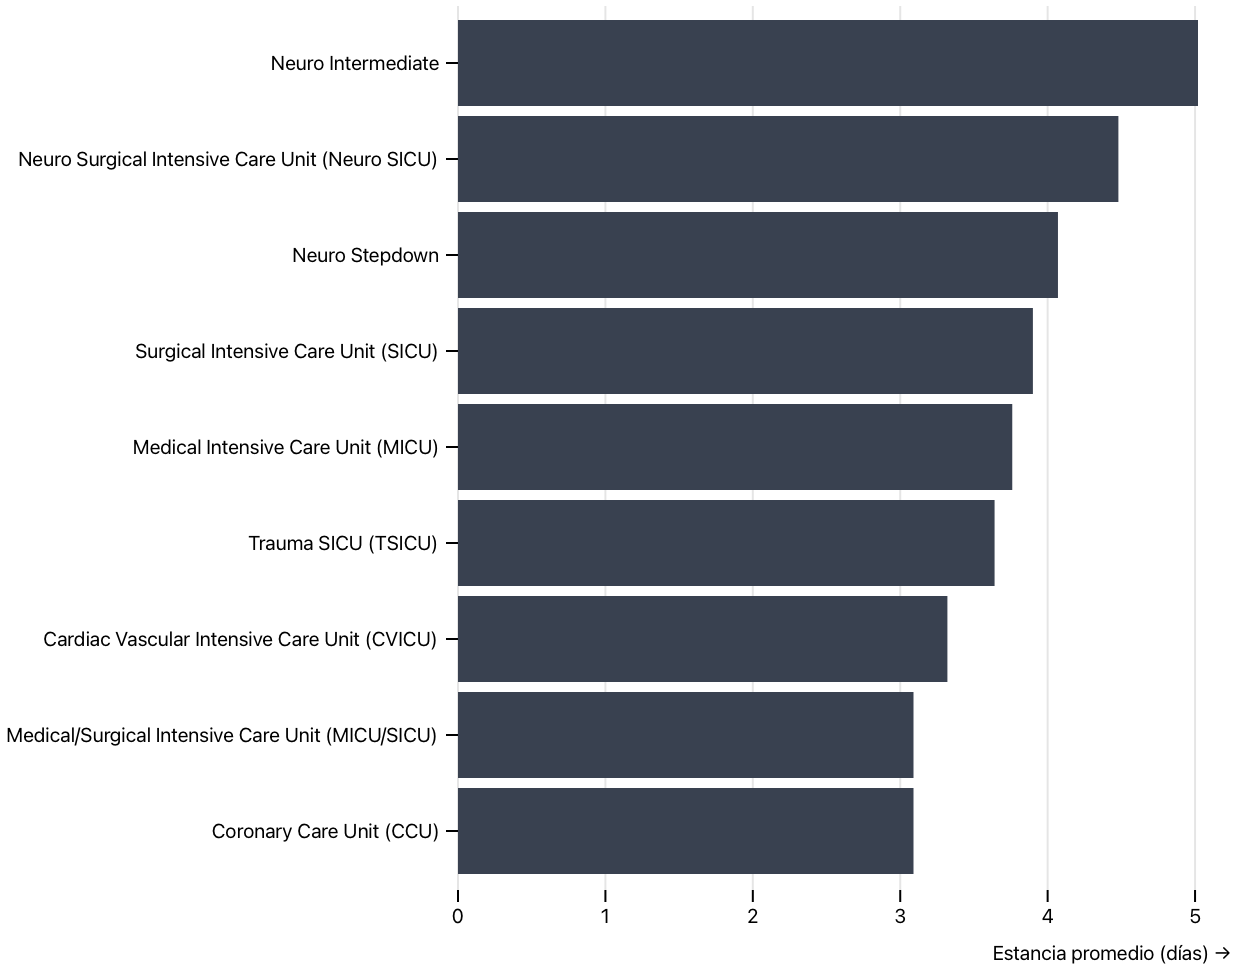
\includegraphics[width=0.65\textwidth]{imagenes/chart1.png}
  \caption{Estancia promedio por unidad UCI}
  \label{fig:chart1}
\end{figure}


\begin{figure}[H]
  \centering
  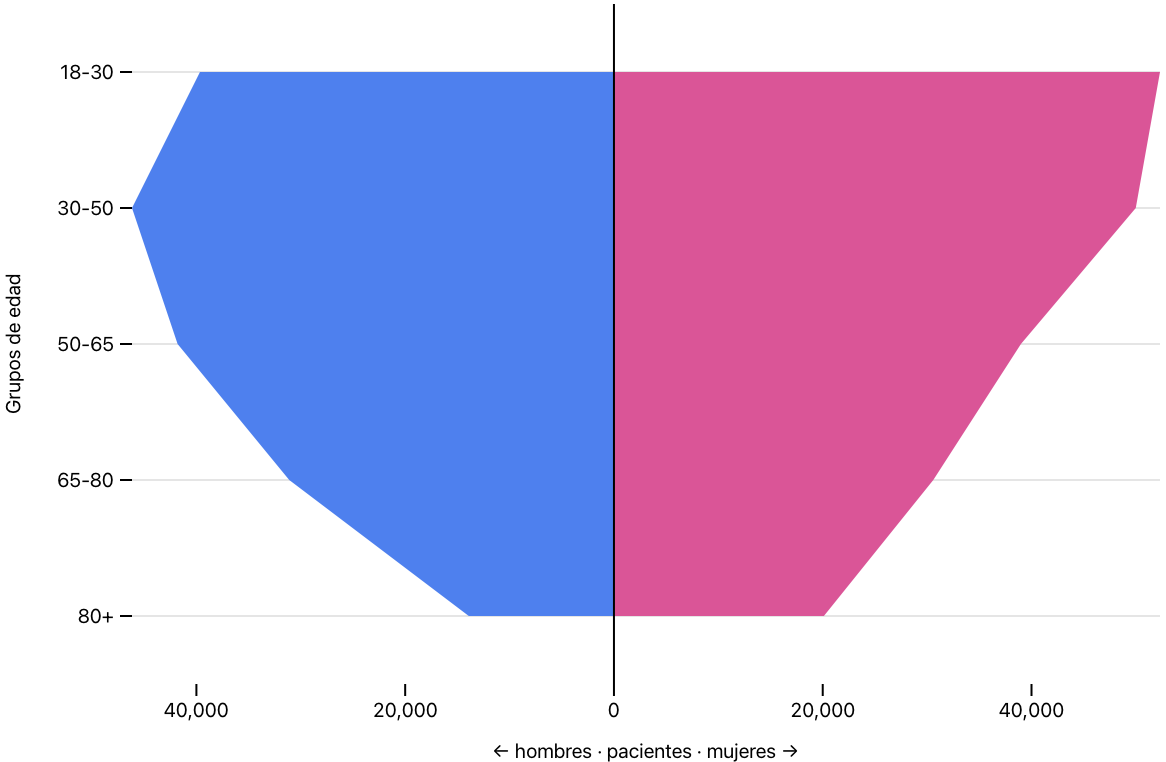
\includegraphics[width=0.65\textwidth]{imagenes/chart2.png}
  \caption{Distribución por edad y género (rangos de edad)}
  \label{fig:chart2}
\end{figure}

\begin{figure}[H]
  \centering
  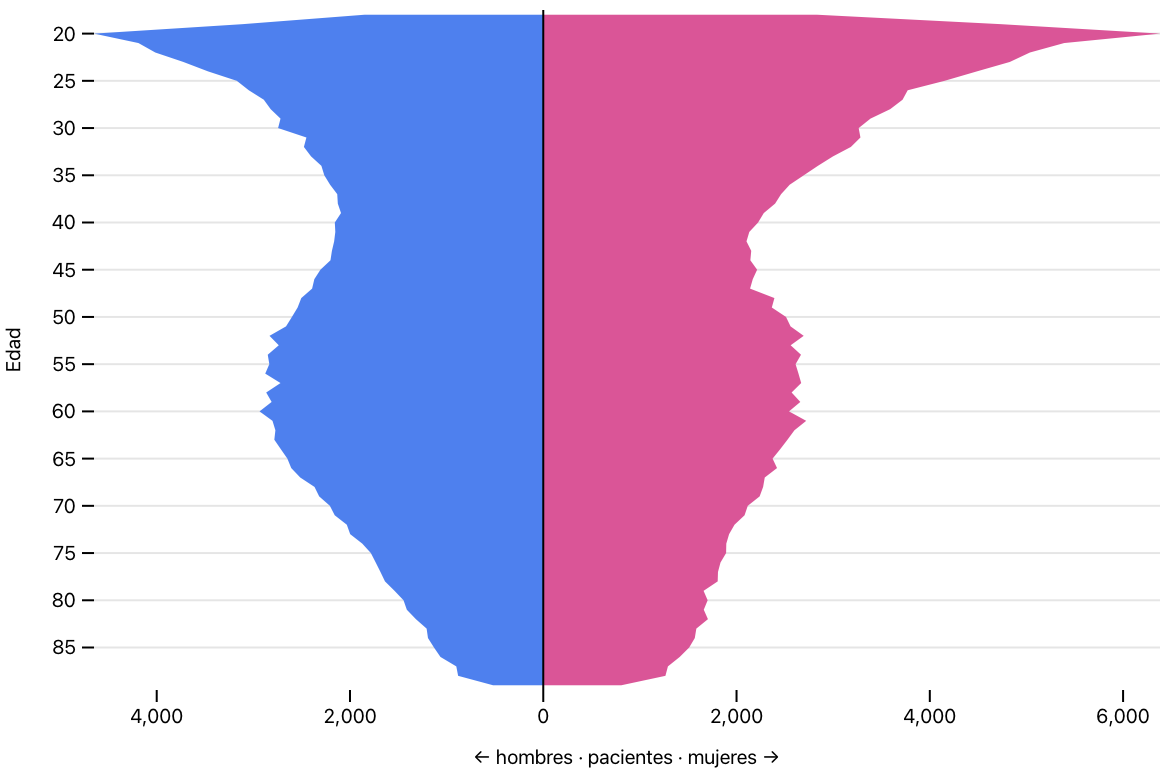
\includegraphics[width=0.65\textwidth]{imagenes/chart3.png}
  \caption{Distribución por edad y género}
  \label{fig:chart3}
\end{figure}






\begin{figure}[H]
  \centering
  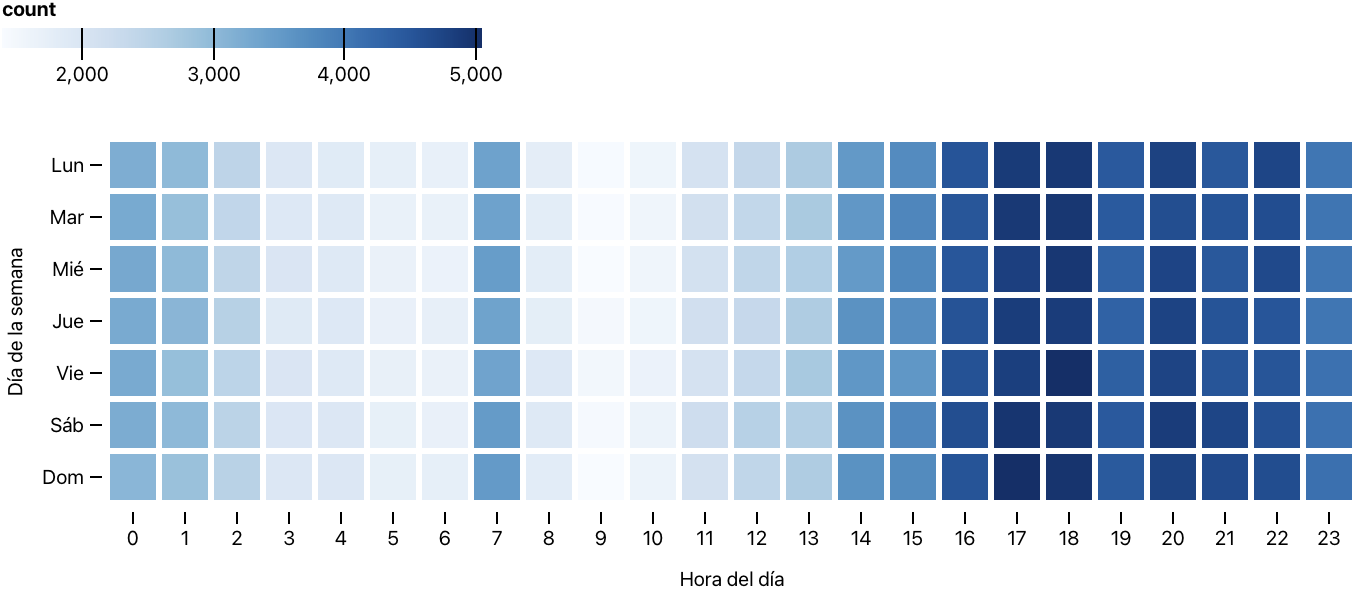
\includegraphics[width=0.8\textwidth]{imagenes/chart4.png}
  \caption{Heatmap de ingresos por hora y día de la semana}
  \label{fig:chart4}
\end{figure}


\begin{figure}[H]
  \centering
  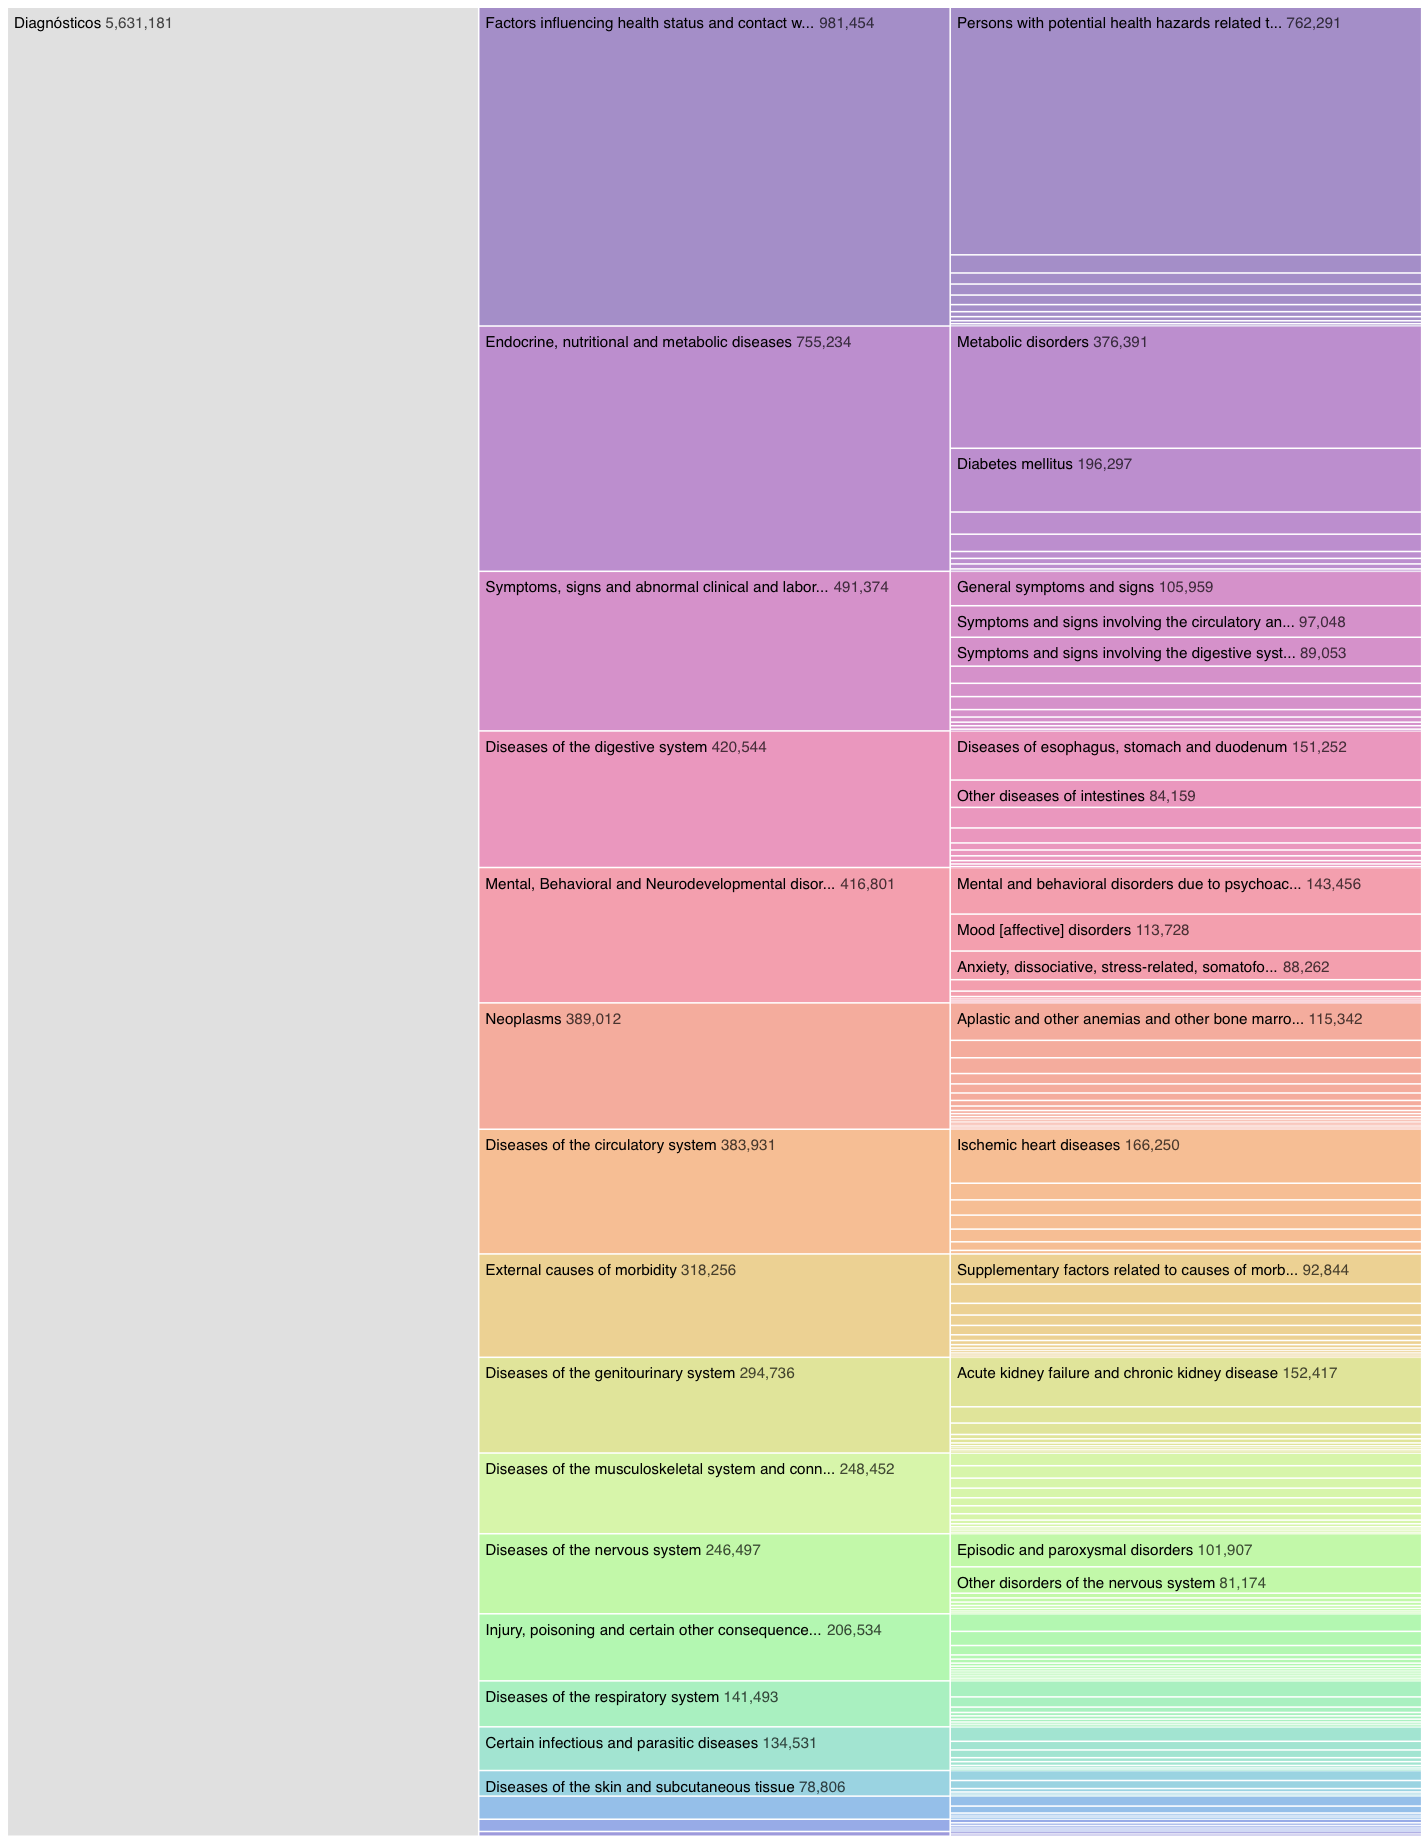
\includegraphics[width=0.88\textwidth]{imagenes/chart5.png}
  \caption{Zoomable icicle chart de diagnósticos por categoría}
  \label{fig:chart5}
\end{figure}

@todo: hablar de cada grafico la info que aporta?

@todo: explicar como seria el proceso de agregar un grafico nuevo?